% !TeX root = ../BA_main_englisch.tex
% !TeX spellcheck = en_GB
In this section we examine the higherdimensional case of $N=5$.
As the data set with $\rho_0 = \ket{+} \bra{+}$, the eigenstate of the drive Hamiltonian, performed best in the previous section, we focus our attention on this case.
We compare the efficiency of a fully connected ANN (FCANN) to a unidirectional and bidirectional LSTM to analyse the effect of different architectures on the predictive power in our setting.
Both LSTM networks have the same architecture, bar the bi-directionality.
Before entering the LSTM cell, each embedded $\ket{\psi_D}$ passes through a two layer FCANN to increase the input dimensionality. 
After passing the LSTM a single layer FCANN is applied to the output to produce the embedding size to recover $\ket{\psi_T}$.
The third network uses three fully connected layers, the size of which is selected to approximately match the amount of trainable parameters of the bidirectional LSTM.

We use Bayesian optimisation implemented by \cite{wandb} to tune model hyperparameters.
The test data efficiency as well as the amount of trainable parameters are presented in table \ref{n5efftable}.

\begin{table}[h]
	\centering
	\begin{tabular}{ c | c | c}
		Network Architecture & $\eta_{test} \ [\%]$  & \# Parameters \\
		\hline
		FCANN & 19.3 & 8,086,020 \\
		Bidirectional LSTM & 33.1 & 7,700,222 \\
		Unidirectional LSTM & 19.5 & 3,206,990\\
	\end{tabular}
	\caption{Efficiencies $\eta$ on the test data for model architectures with given number of trainable parameters.}
	\label{n5efftable}
\end{table}

\begin{figure}
	\centering
	\begin{subfigure}{0.32\textwidth}
		\centering
		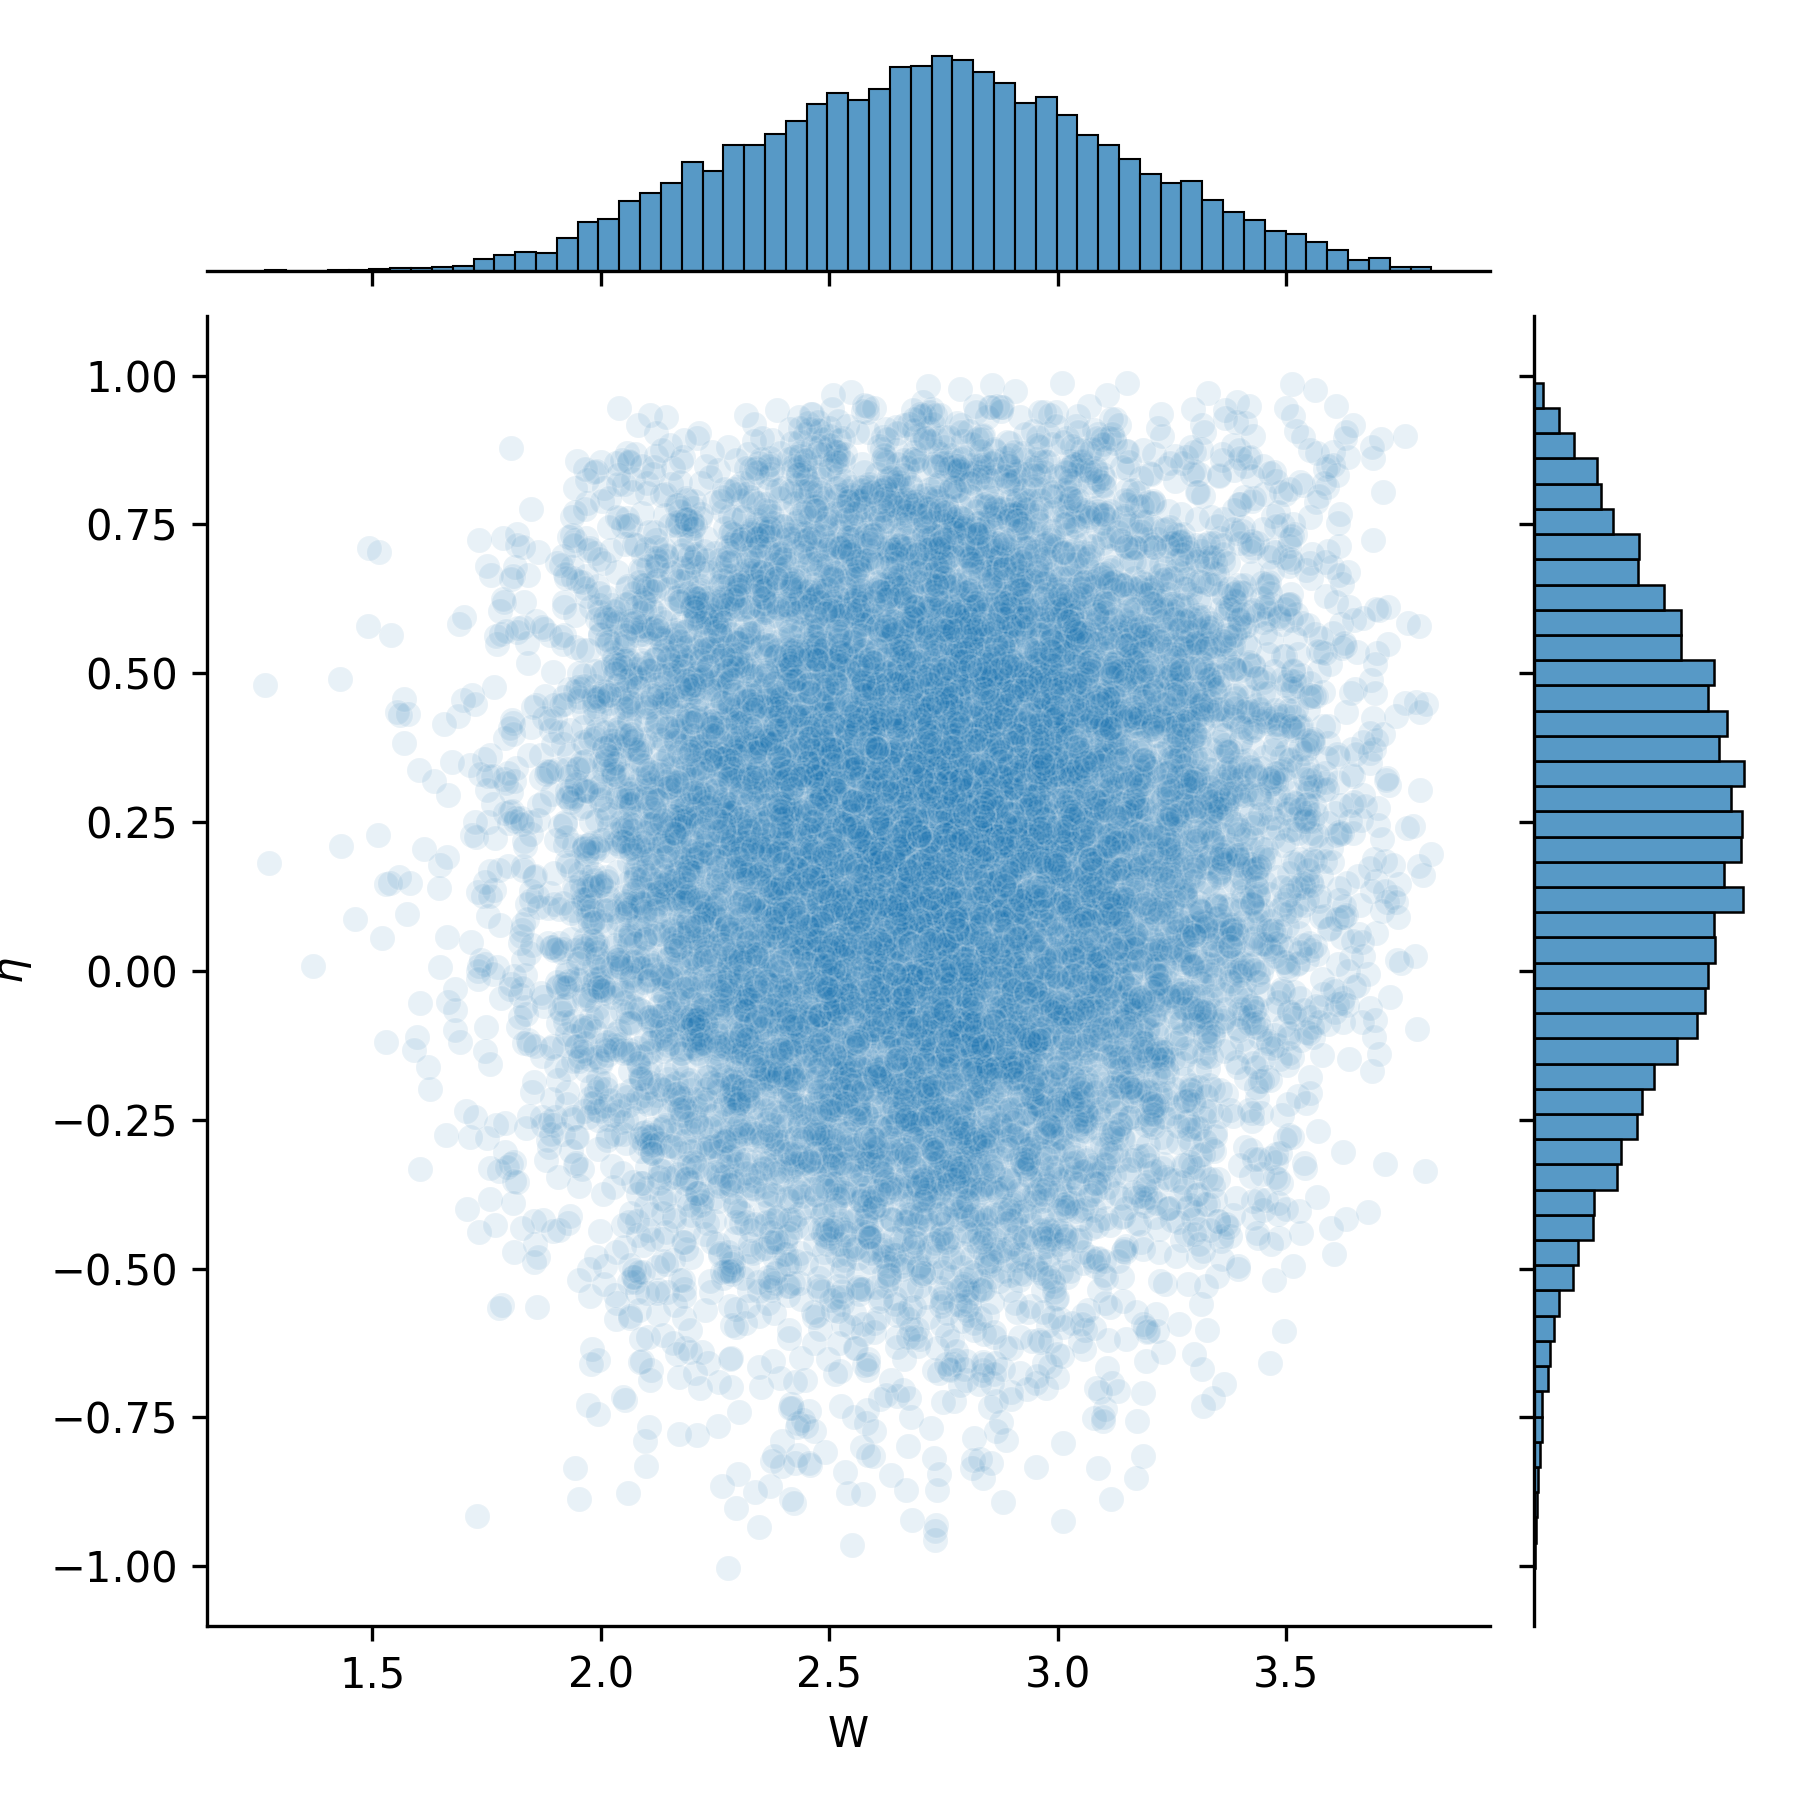
\includegraphics[width=\textwidth]{img/work_dist_n5_eigen_ann}
		\caption{FCANN}
		\label{}
	\end{subfigure}
	\begin{subfigure}{0.32\textwidth}
		\centering
		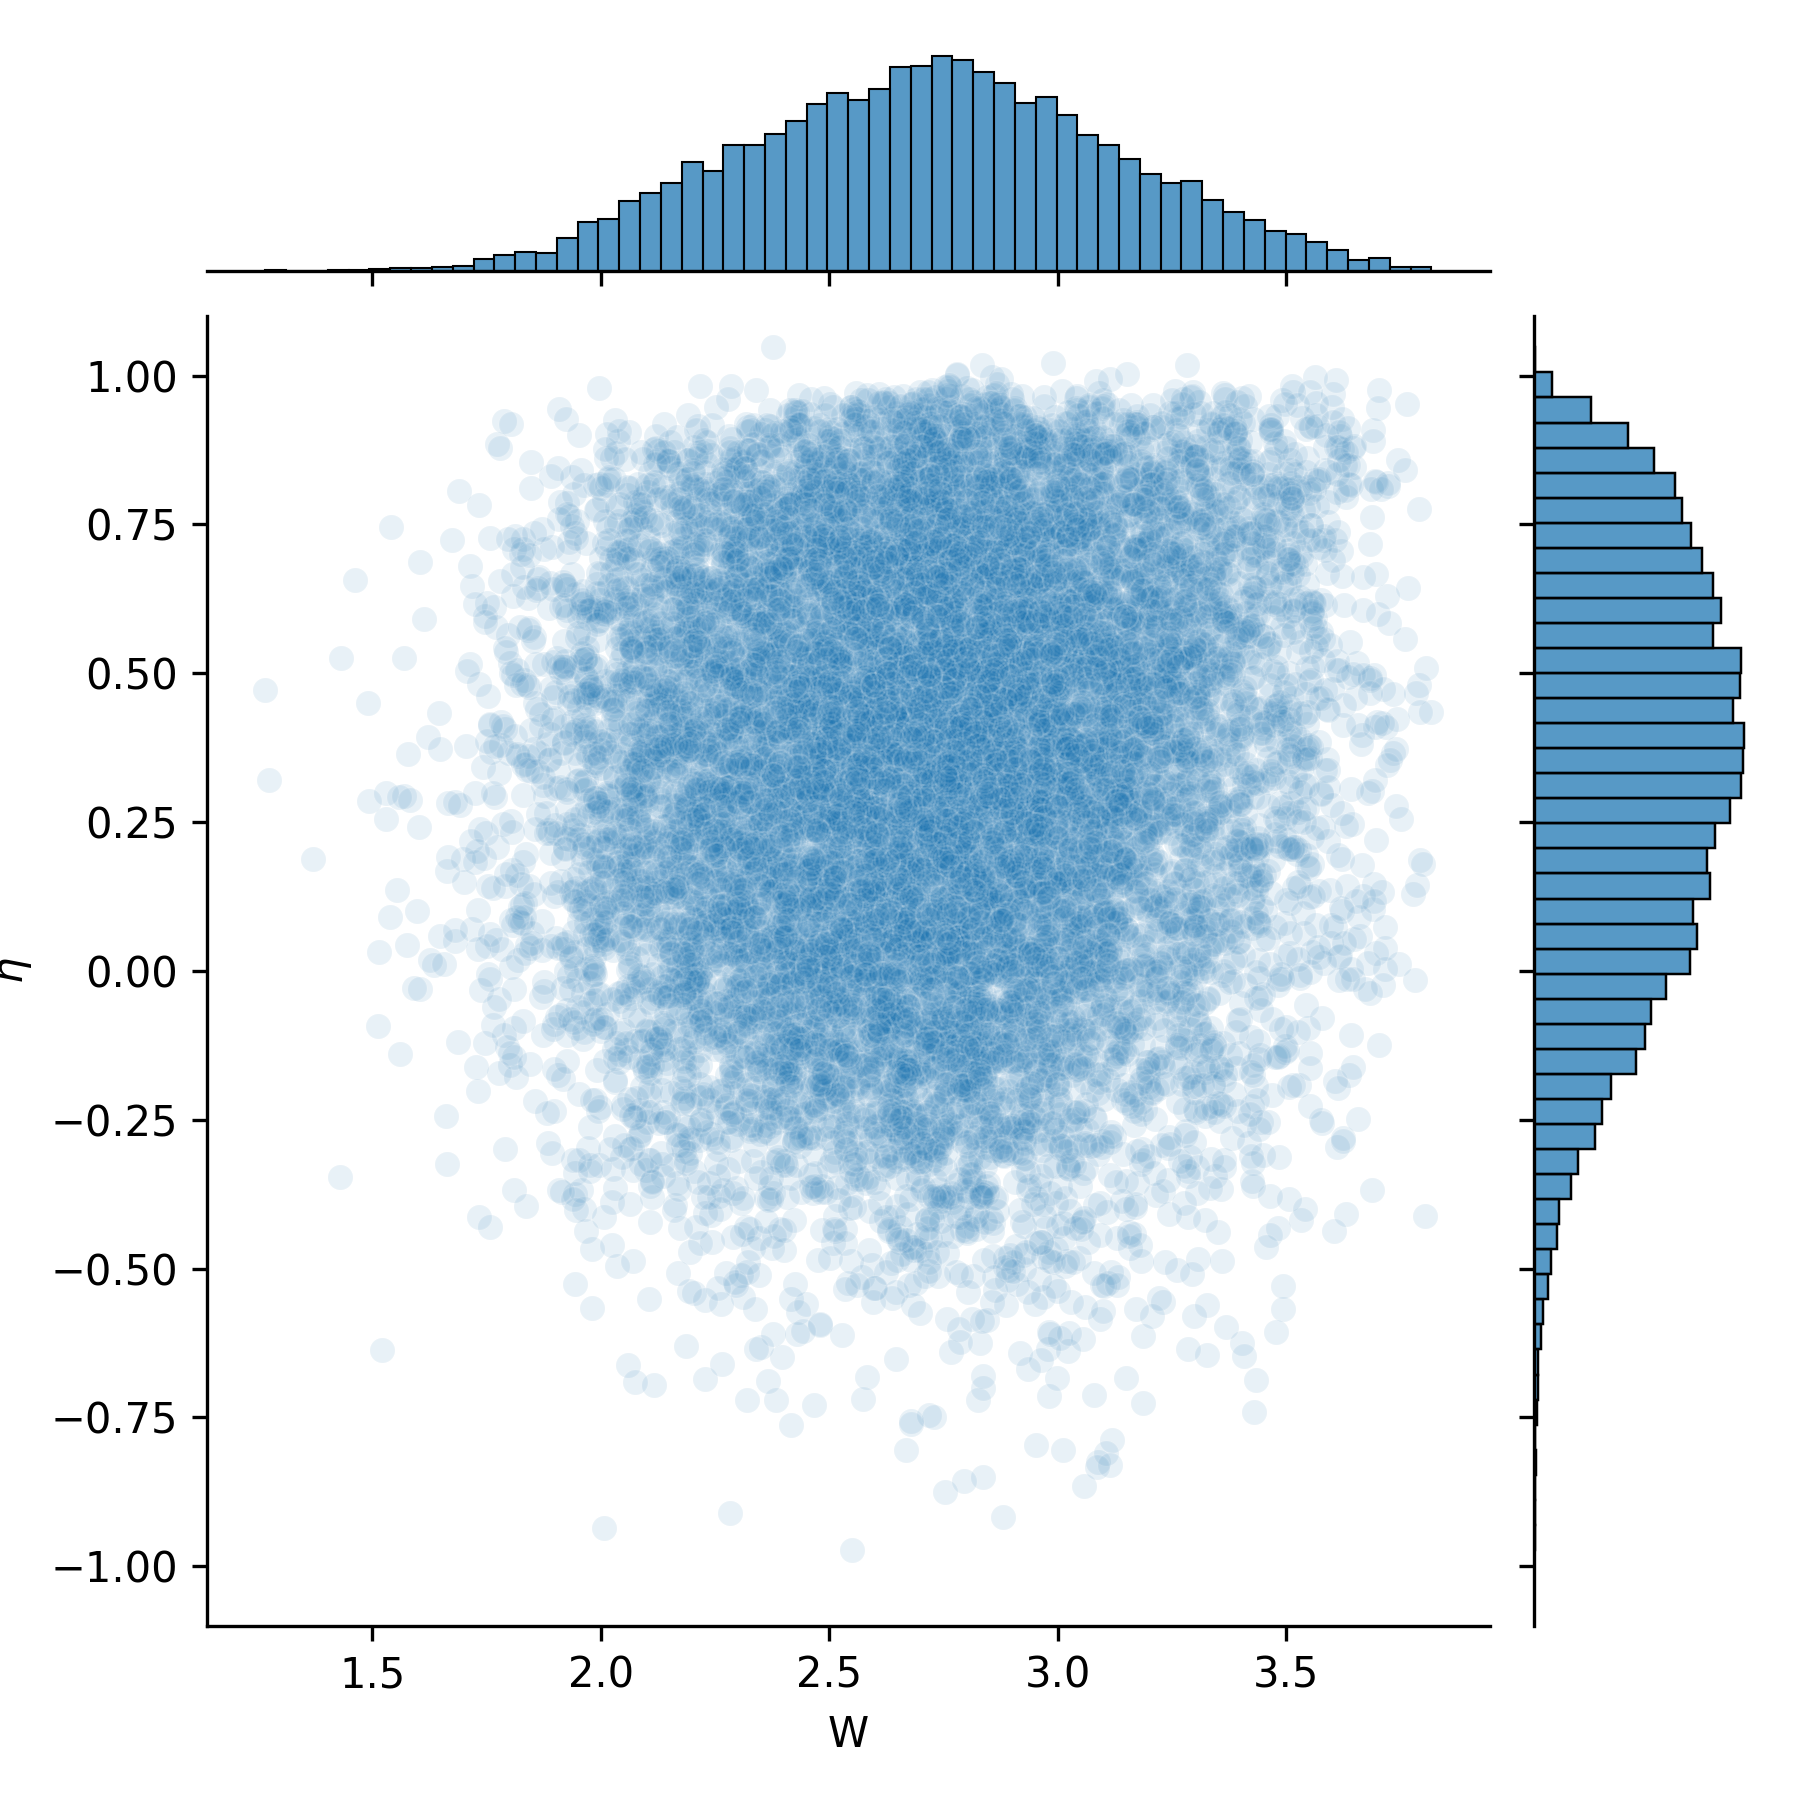
\includegraphics[width=\textwidth]{img/work_dist_n5_eigen_bi}
		\caption{Bidir. LSTM}
		\label{}
	\end{subfigure}
	\begin{subfigure}{0.32\textwidth}
	\centering
	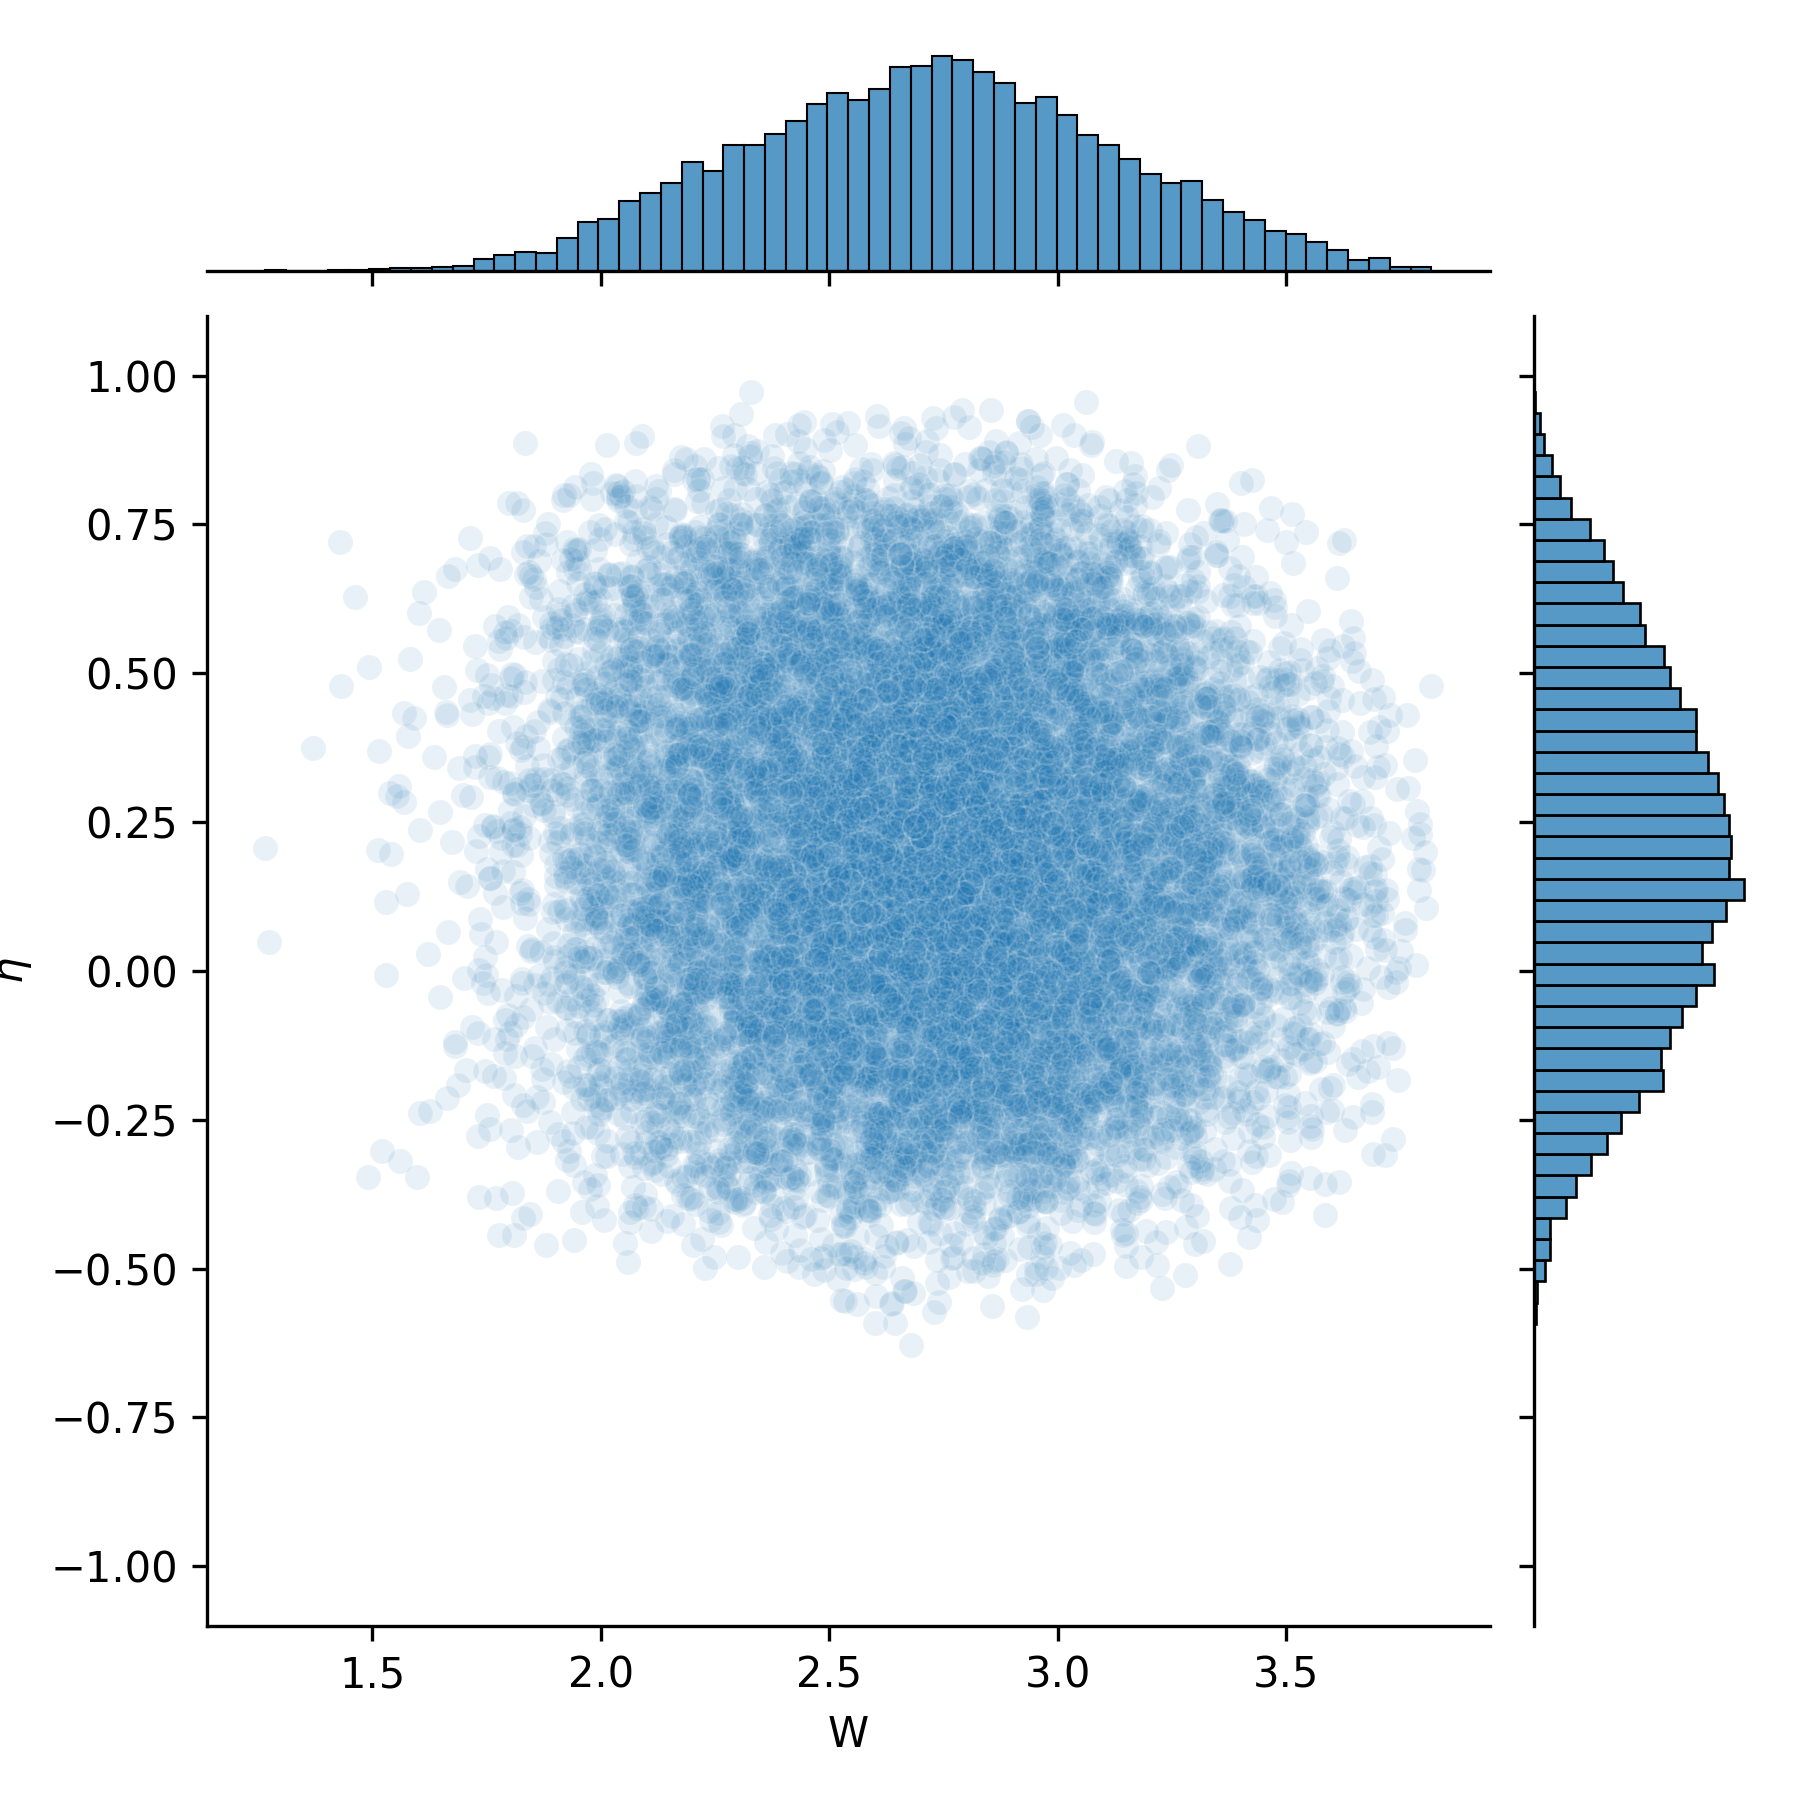
\includegraphics[width=\textwidth]{img/work_dist_n5_eigen_uni}
	\caption{Unidir. LSTM}
	\label{}
\end{subfigure}
	\caption{We plot the efficiency $\eta$ of each data point in the test set over its optimal work output $W$ for the three network architectures and $\rho_0 = \ket{+}\bra{+}$. The top and right plots on each graph are histograms for $W$ and $\eta$ respectively.}
	\label{}
\end{figure}

\subsection{Noise resistance}
Besides the efficiency of the networks the resistance of their predictions to noise is also of interest.
We create a noisy sequence $\{\ket{\phi_j}\}$ of N qubits from $\{\ket{\psi_j}\}$ using
\begin{align*}
	\ket{\phi_j} = e^{-i H_j \tau} \ket{\psi_j}, \ \forall j \in [1, N].
\end{align*}
$H_j$ are randomly generated Hermitian matrices and $\tau$ is a real parameter used to control the strength of the noise.
To quantify the dissimilarity between $\{\ket{\phi_j}\}$ and $\{\ket{\psi_j}\}$ we use the fidelity $F$ as defined in \cite{10.5555/1972505}:
\begin{align*}
	F_{\text{run}}(\{\ket{\phi_j}\}, \{\ket{\psi_j}\}) = \prod_j F(\ket{\phi_j}, \ket{\psi_j}) = \prod_j \abs{\bra{\phi_j}\ket{\psi_j}}.
\end{align*}
